% Appendix X

\chapter{RICH efficiencies}\label{app:RICH}

%----------------------------------------------------------------------------------------

In this appendix the results for the RICH particle identification efficiency are shown in Figs. \ref{pic:Effpim} to \ref{pic:Effpm} for $\pi^-$, $K^-$, $p$ and $\bar{p}$ for the various particle types and charges. In each figure, the momentum dependence for the different angular bins is shown. The efficiencies are weakly dependent on the angle, while it is more strongly correlated with the momentum, especially in the region near the threshold.

\begin{figure}[!p]
  \centering
	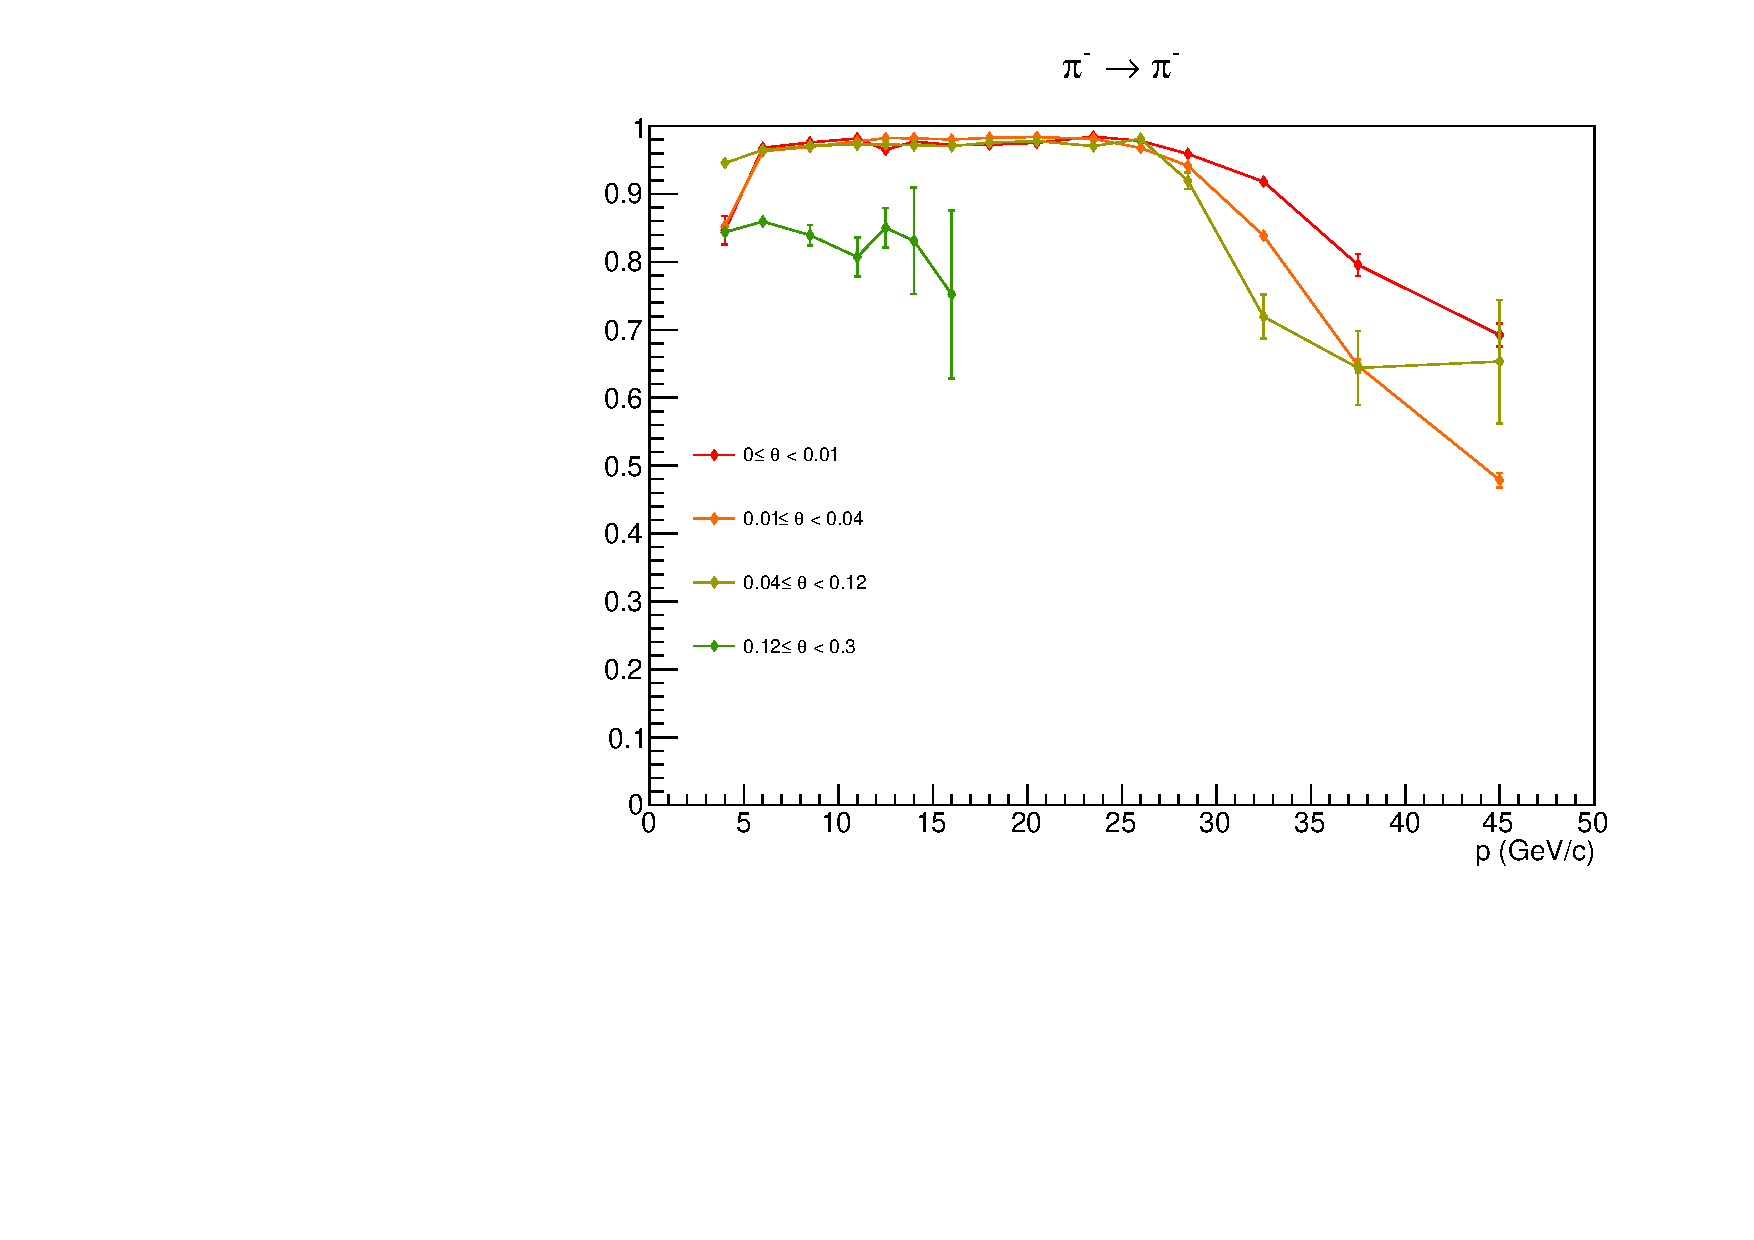
\includegraphics[scale=0.38]{./gfx/pim_pi.pdf}
  \includegraphics[scale=0.38]{./gfx/pim_K.pdf}
  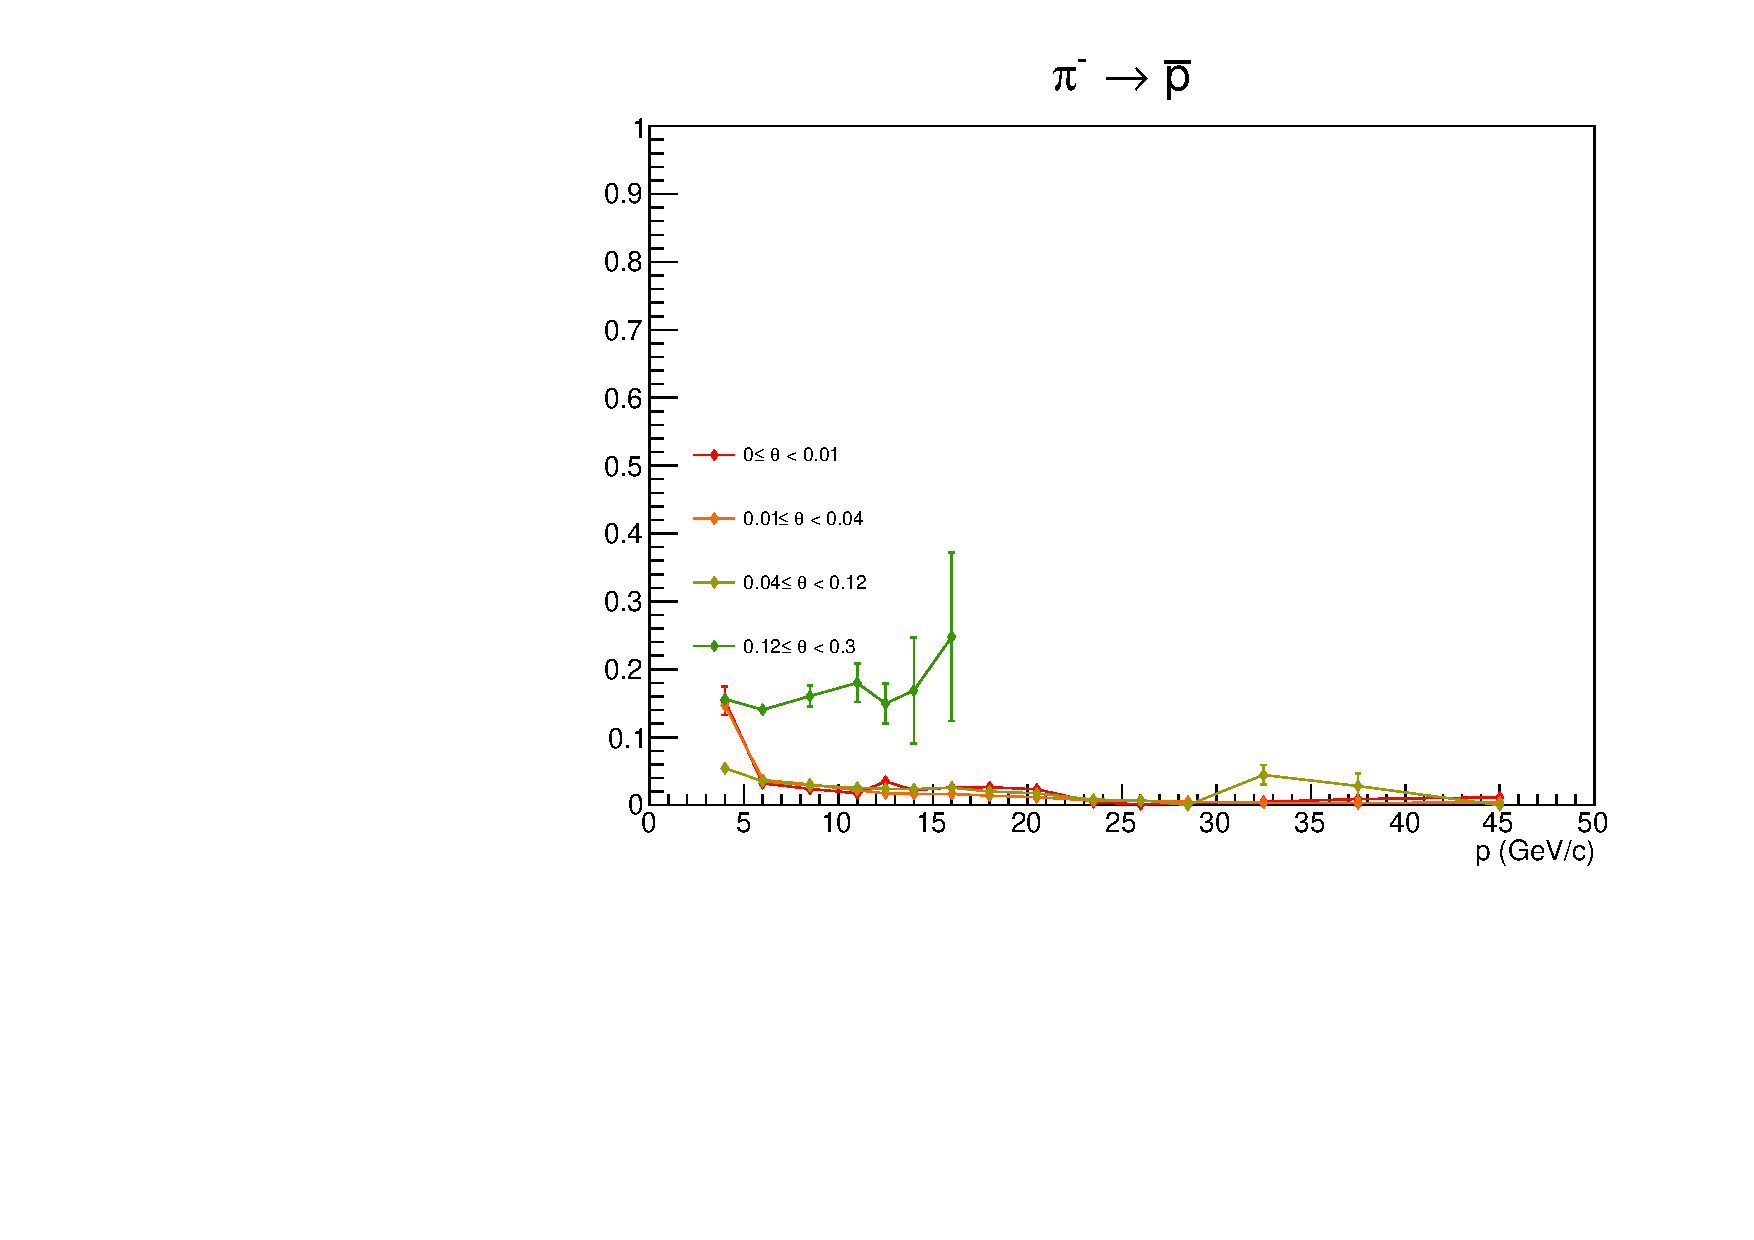
\includegraphics[scale=0.38]{./gfx/pim_p.pdf}
  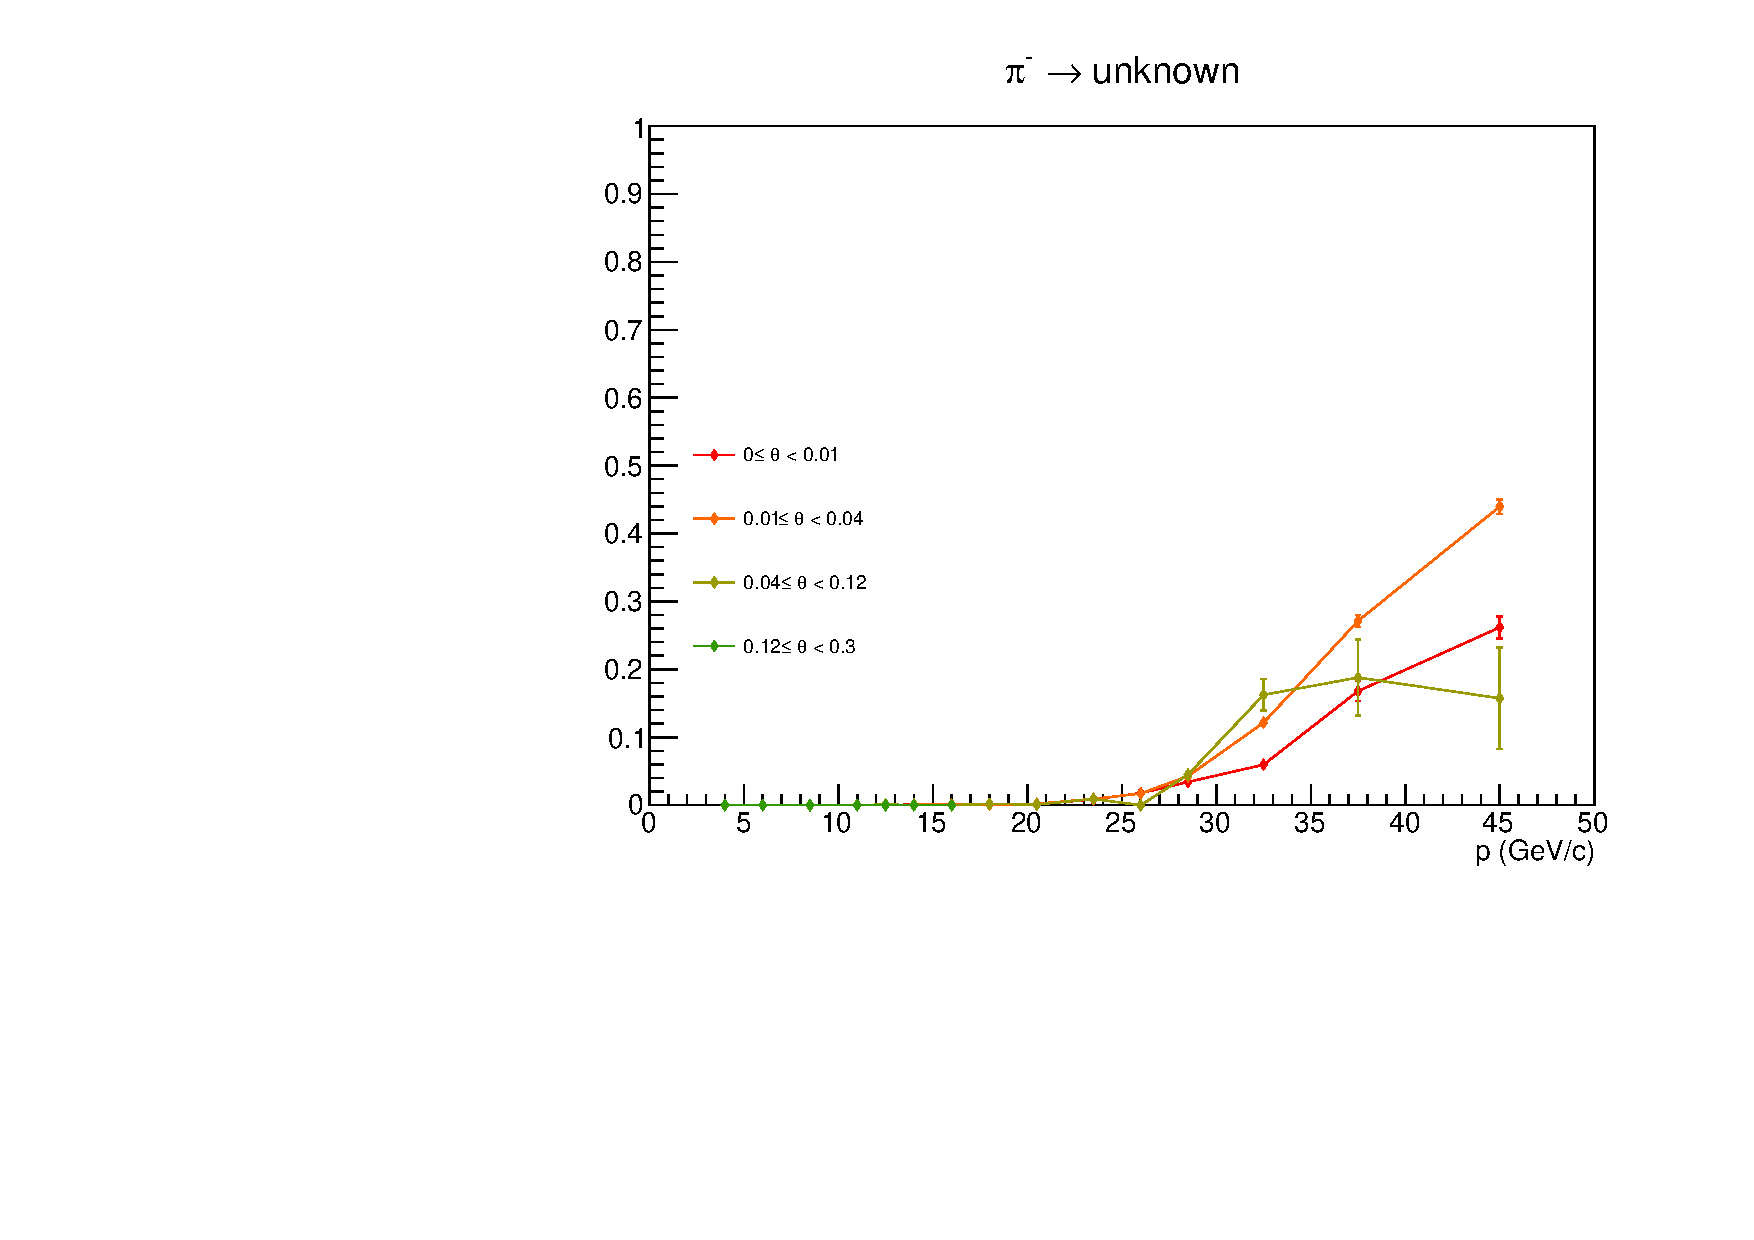
\includegraphics[scale=0.38]{./gfx/pim_u.pdf}
	\caption{Identification probabilities $\epsilon(p \rightarrow j)$ for $\pi^-$.}
	\label{pic:Effpim}
\end{figure}


\begin{figure}[!p]
  \centering
	\includegraphics[scale=0.38]{./gfx/Km_pi.pdf}
  \includegraphics[scale=0.38]{./gfx/Km_K.pdf}
  \includegraphics[scale=0.38]{./gfx/Km_p.pdf}
  \includegraphics[scale=0.38]{./gfx/Km_u.pdf}
	\caption{Identification probabilities $\epsilon(p \rightarrow j)$ for $K^-$.}
	\label{pic:Effkm}
\end{figure}

\begin{figure}[!p]
  \centering
	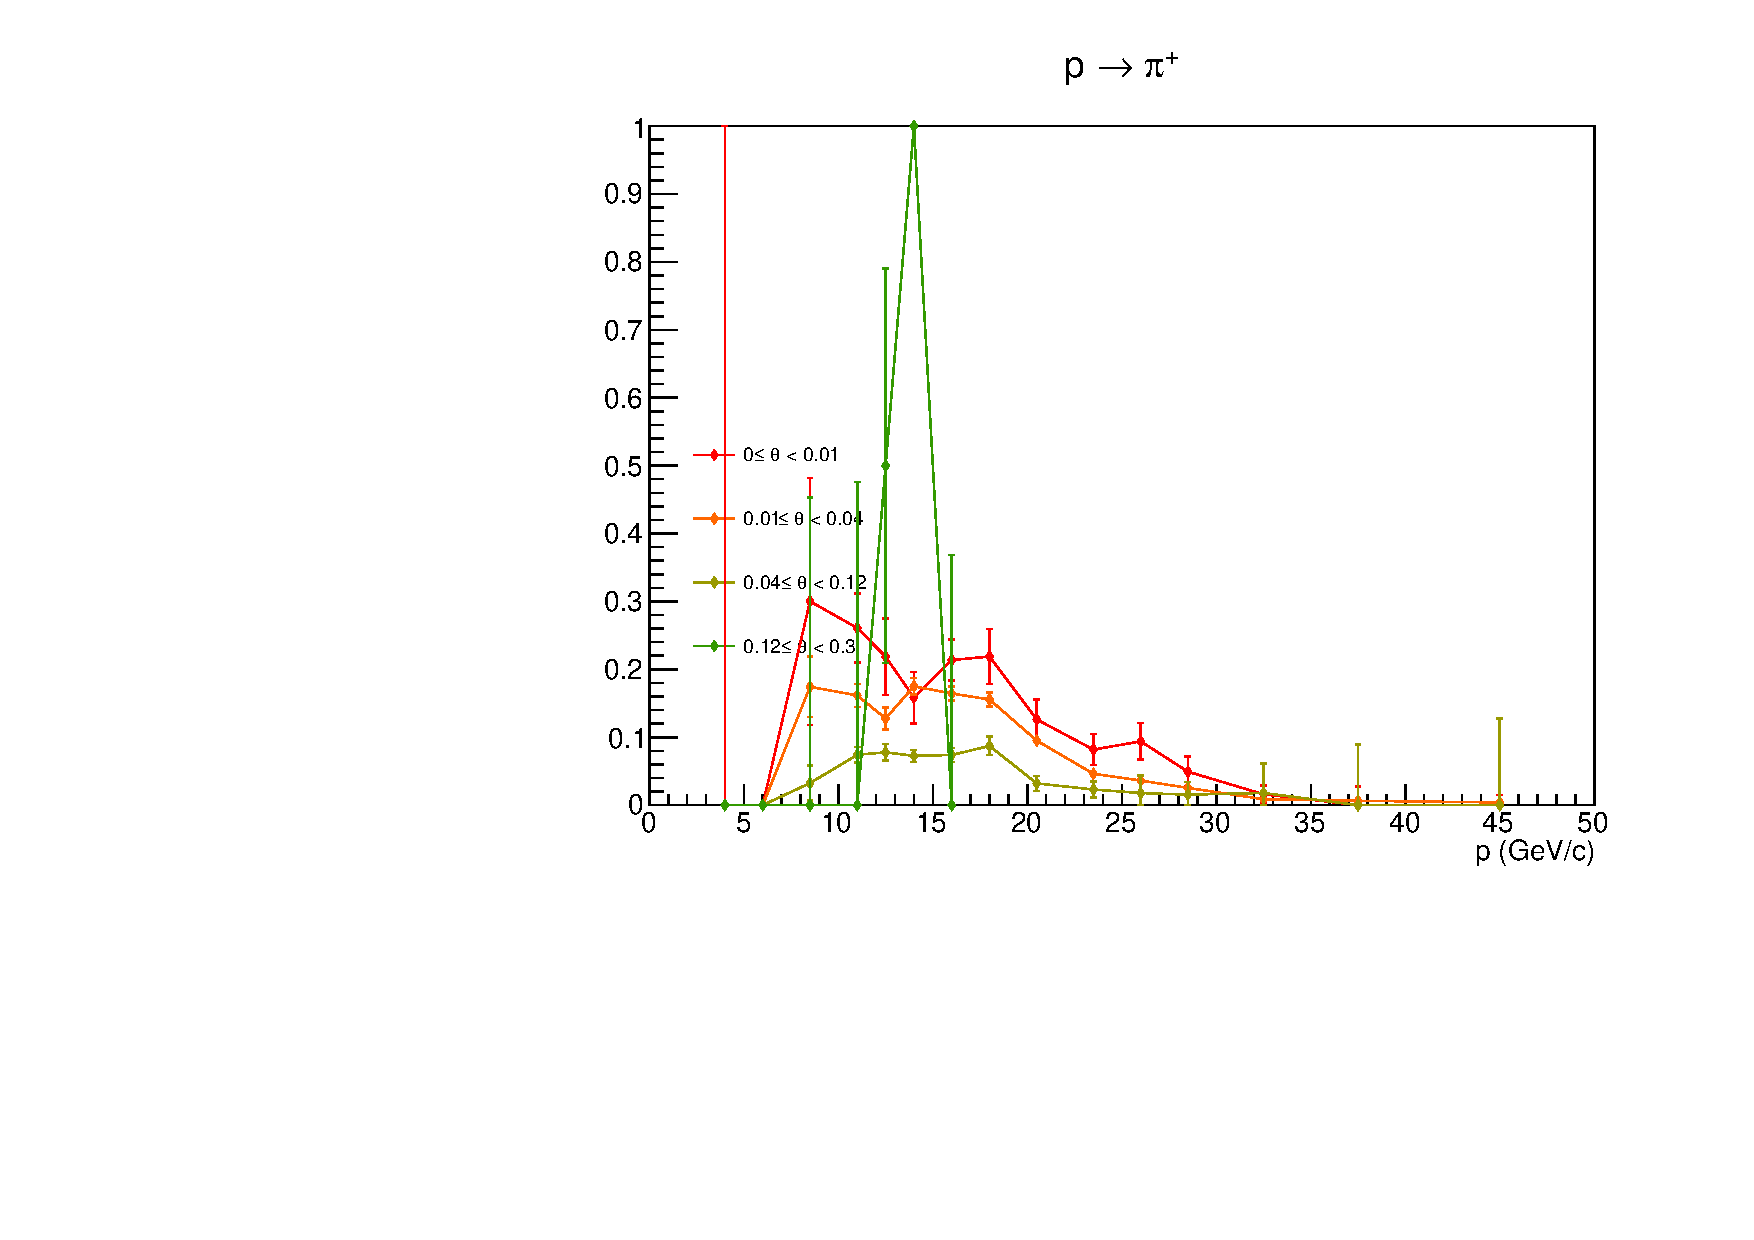
\includegraphics[scale=0.38]{./gfx/pp_pi.pdf}
  \includegraphics[scale=0.38]{./gfx/pp_K.pdf}
  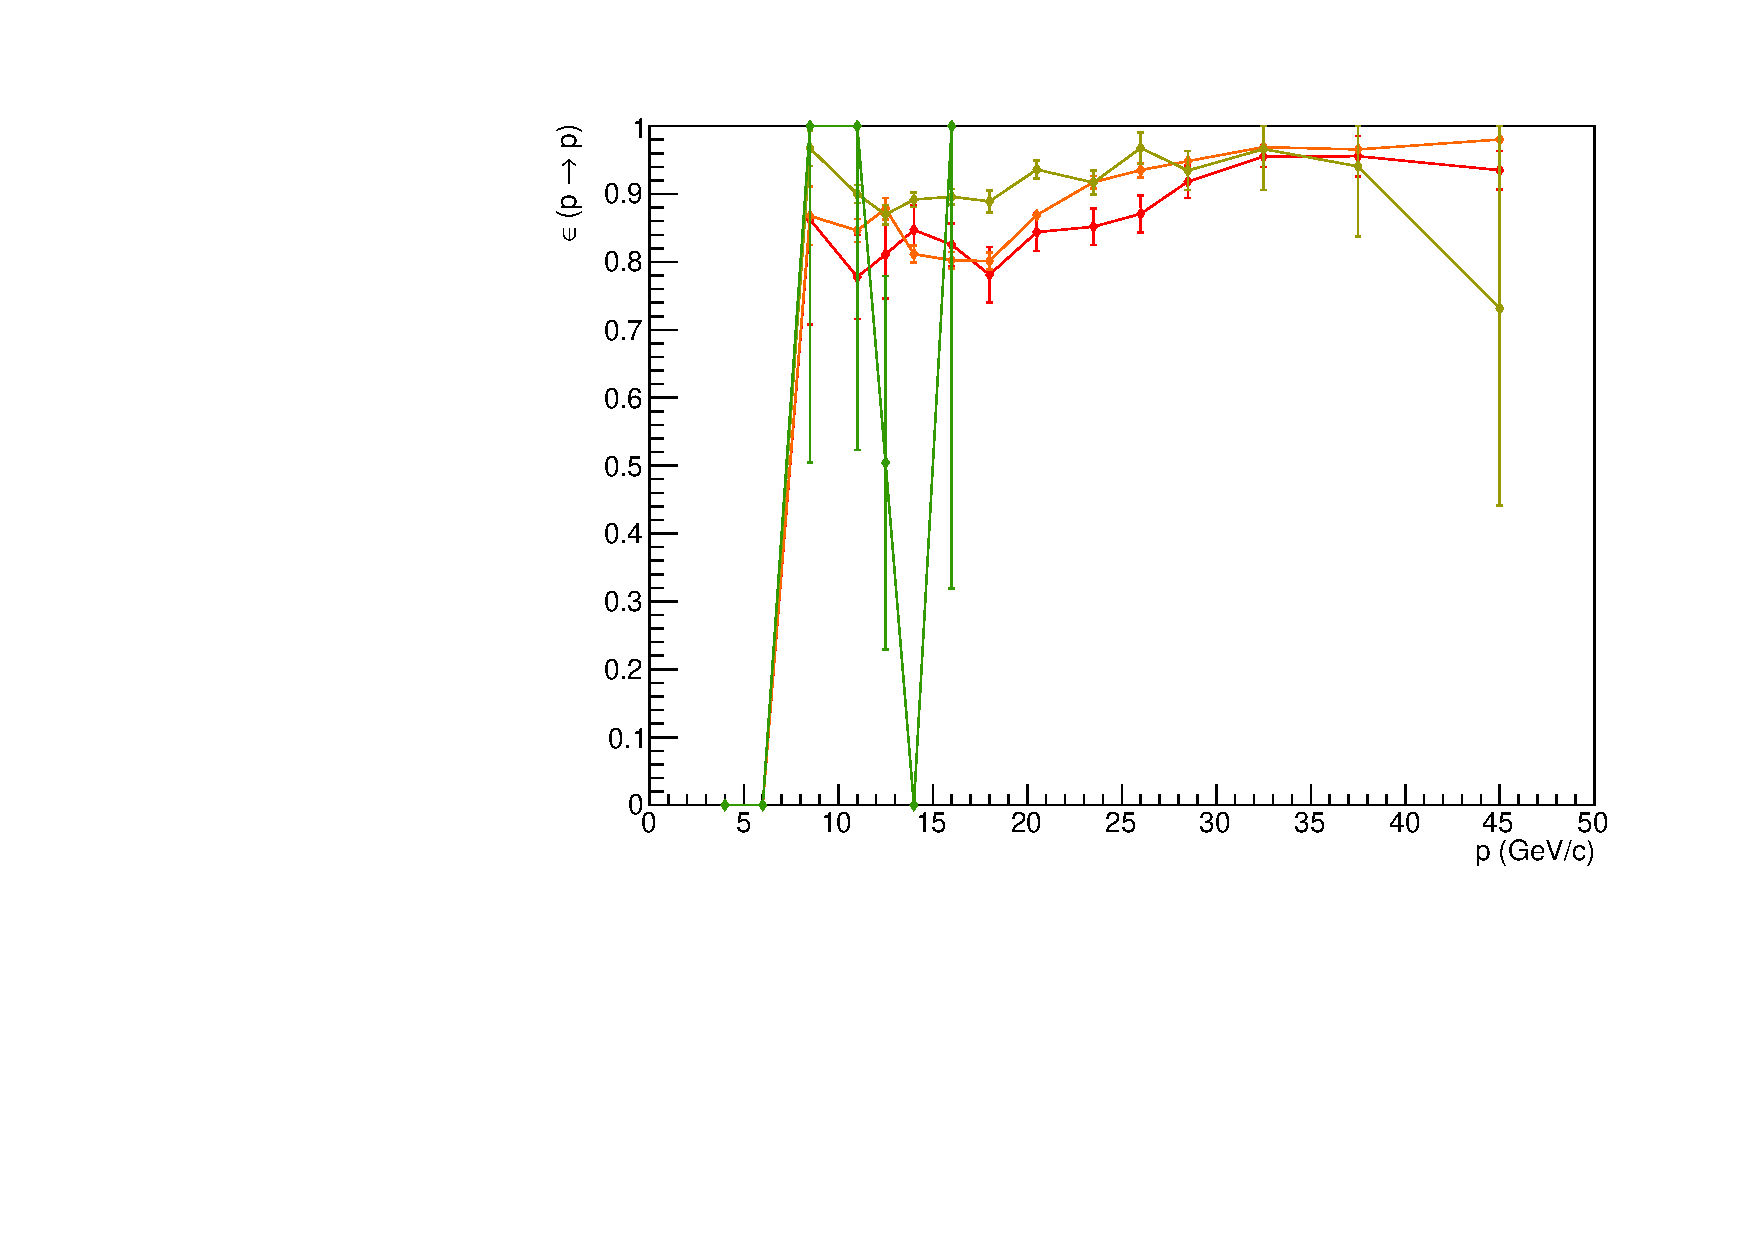
\includegraphics[scale=0.38]{./gfx/pp_p.pdf}
  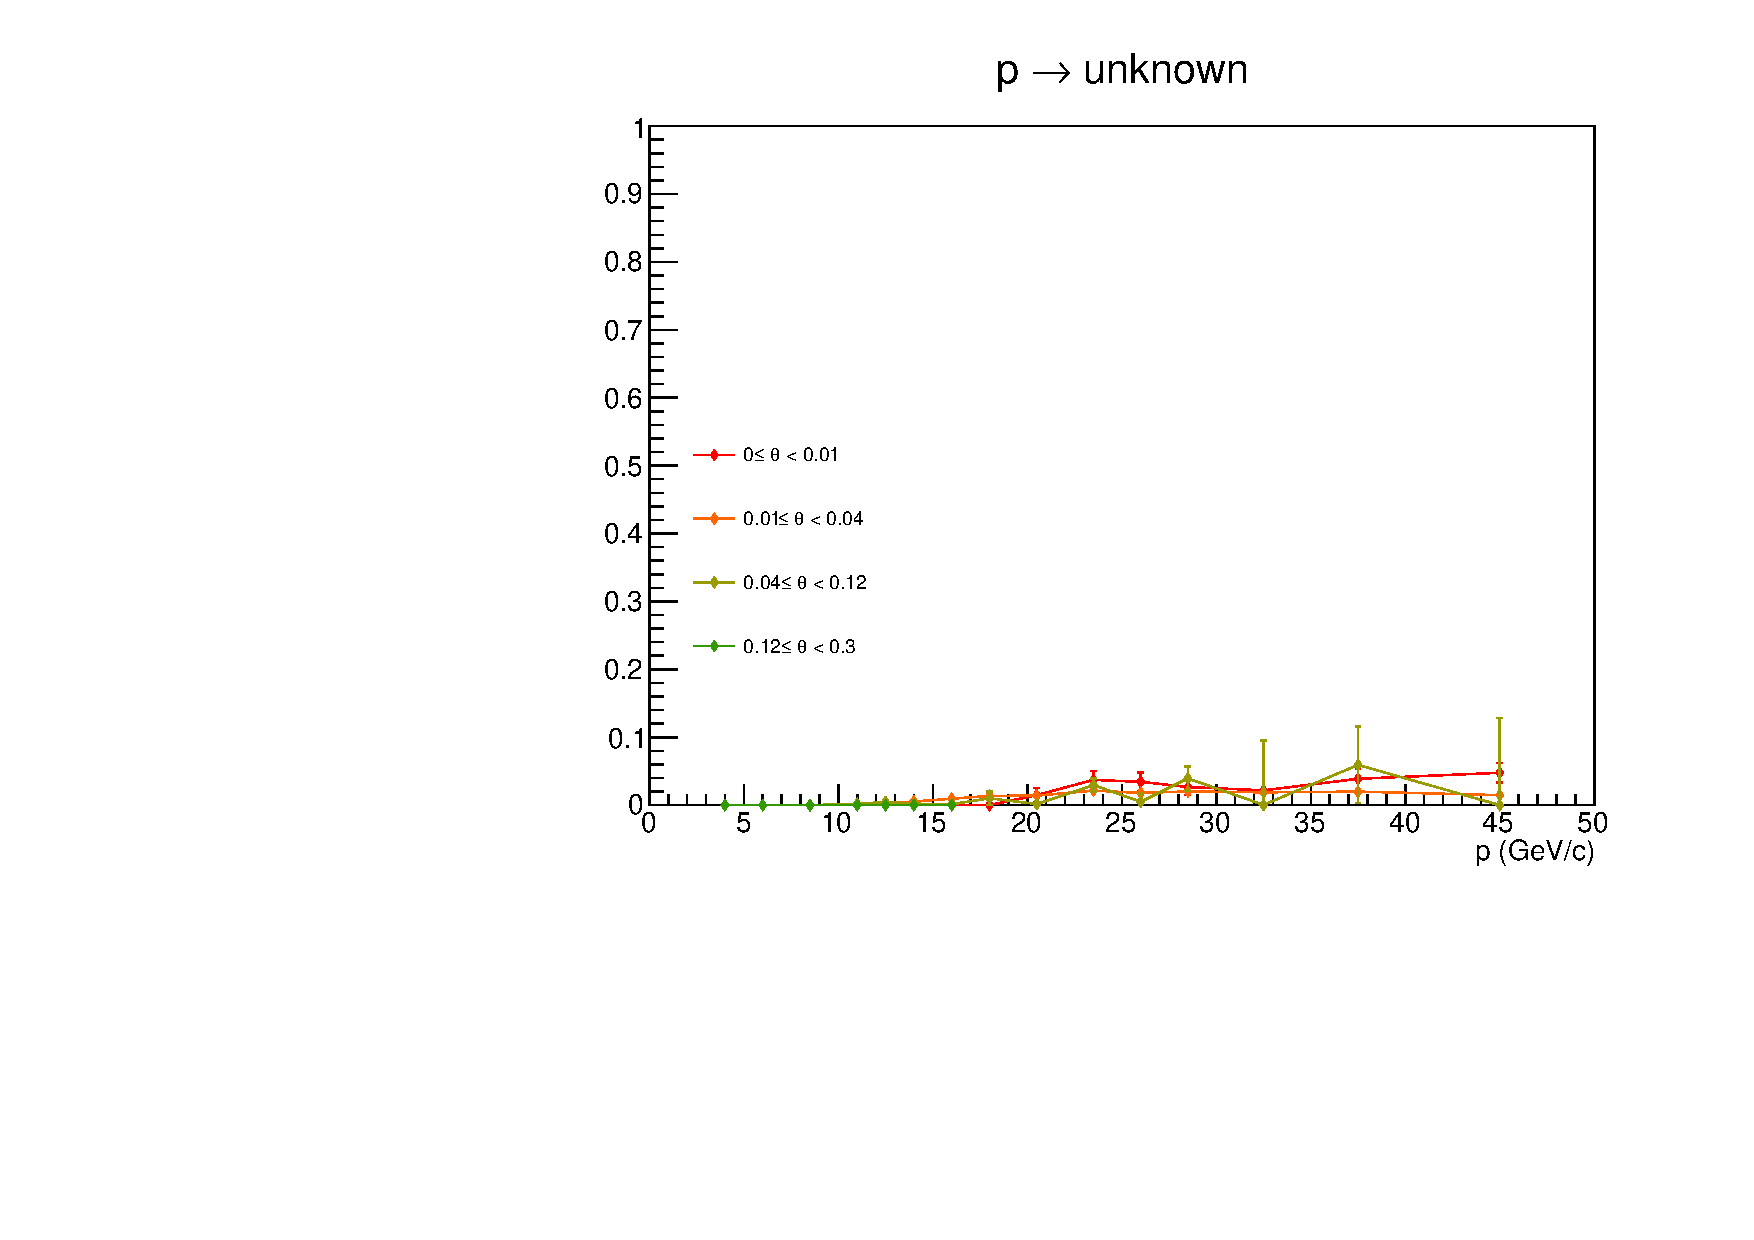
\includegraphics[scale=0.38]{./gfx/pp_u.pdf}
	\caption{Identification probabilities $\epsilon(p \rightarrow j)$ for $p$.}
	\label{pic:Effpp}
\end{figure}

\begin{figure}[!p]
  \centering
	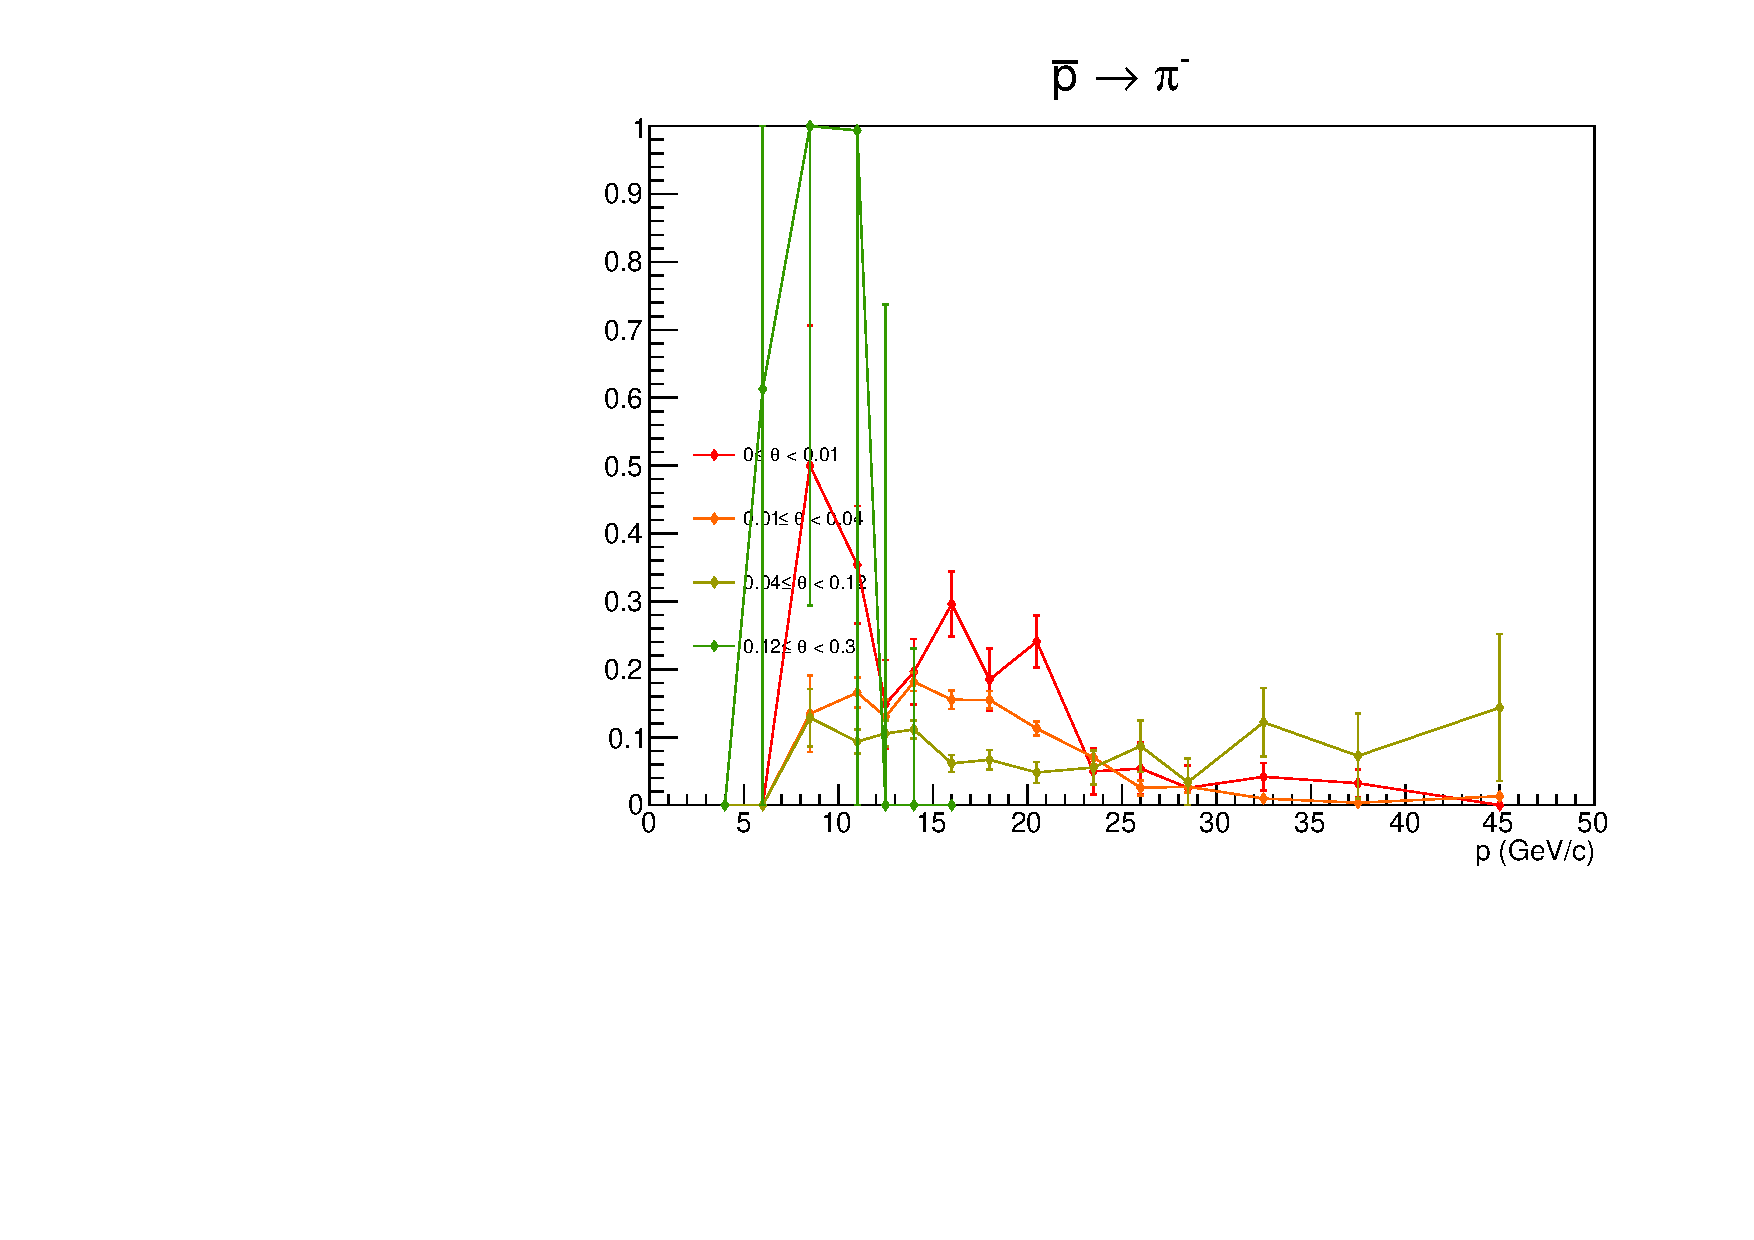
\includegraphics[scale=0.38]{./gfx/pm_pi.pdf}
  \includegraphics[scale=0.38]{./gfx/pm_K.pdf}
  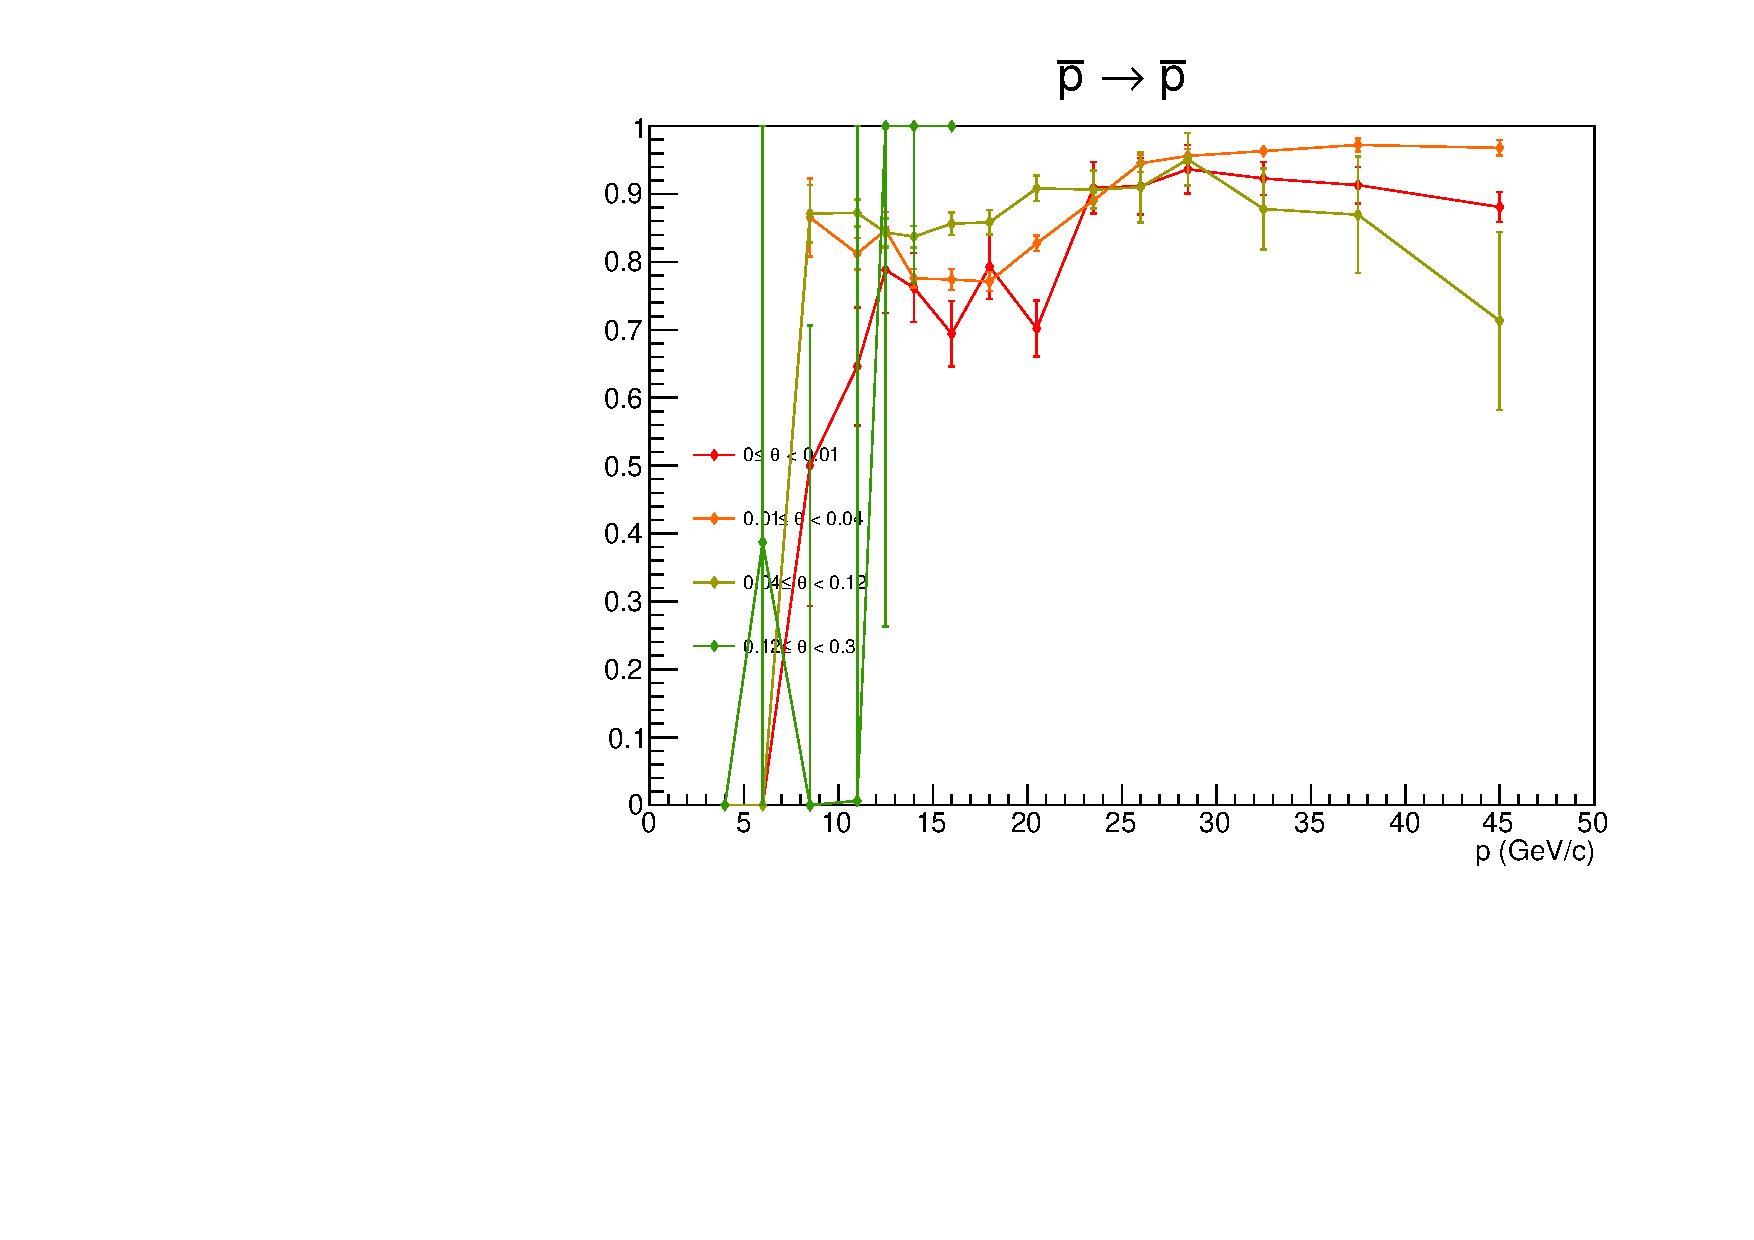
\includegraphics[scale=0.38]{./gfx/pm_p.pdf}
  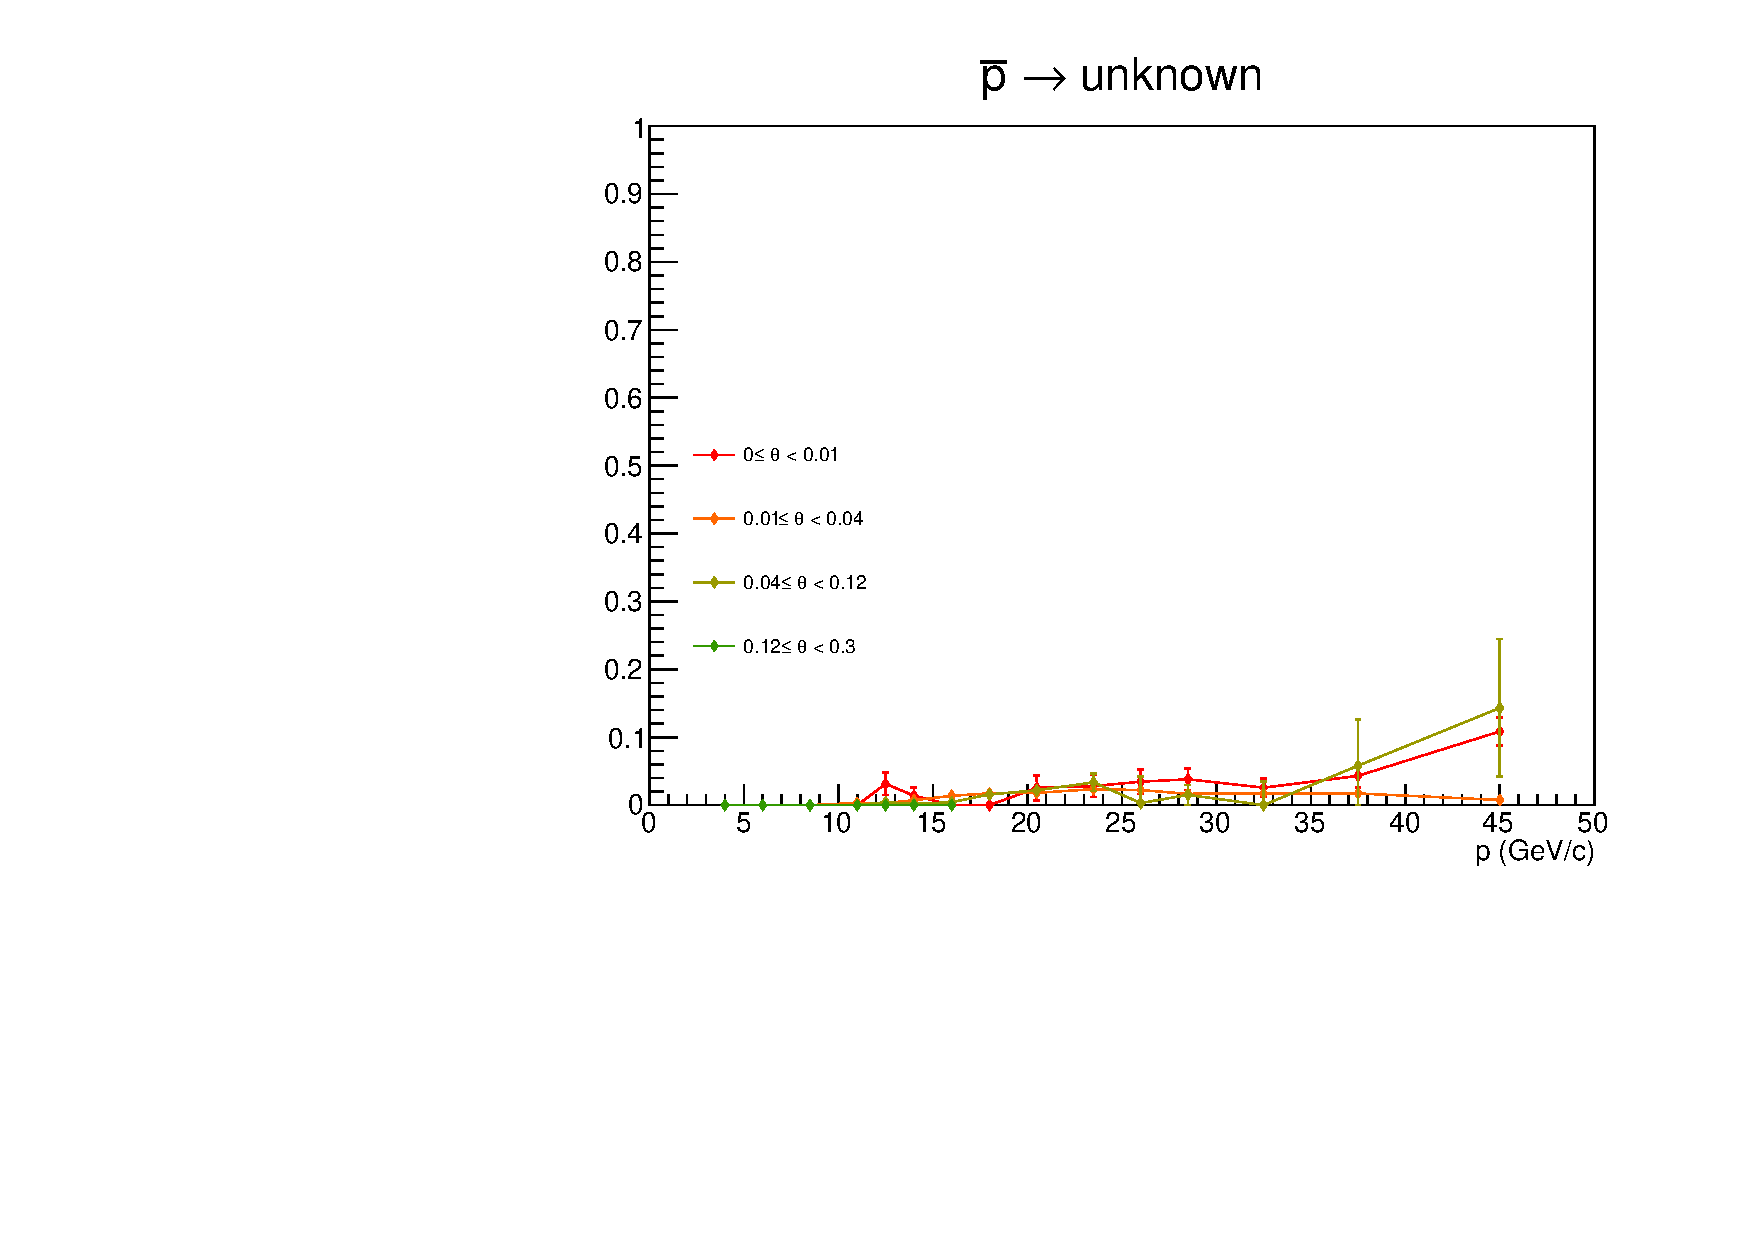
\includegraphics[scale=0.38]{./gfx/pm_u.pdf}
	\caption{Identification probabilities $\epsilon(p \rightarrow j)$ for $\bar{p}$.}
	\label{pic:Effpm}
\end{figure}
